\section{Experiments}
\label{sec:experiments}

Every experiment asks the same operational question: does a student satisfy a
threshold fixed before its capacity is inspected?  The three settings have
different roles.  The image torus has a mathematical ground truth and proves a
minimum rank; the warped Gaussian torus tests neural optimization with
nonconstant variances; MNIST and FashionMNIST test compression, decoded
outputs, and numerical intrinsic paths for learned decoders.

\subsection{An Exact Shared-Trunk Minimum}
\label{sec:controlled-experiment}

\paragraph{Setup.}
We instantiate Section~\ref{sec:exact-task} with $T=128$, $a_j=1/j$, and $Q$
equal to the first 512 two-dimensional DCT atoms in zig-zag order.  The dense
$784\times512$ teacher head, including its bias, uses $402{,}192$ stored
scalars.  A factorized rank-$r$ head uses $r(784+512)+784$.  This count treats
the head as a dense deployed matrix; the analytic DCT construction itself is
of course more compact.

We predeclare two simultaneous requirements,
\begin{equation}
 E_0\le\eta=5\%,
 \qquad
 D_{\rm pair}\le\tau=5\%.
 \label{eq:exact-requirements}
\end{equation}
The exact identity $D_{\rm loc}=D_{\rm pair}$ makes the second condition
computable without a path solver.  Displayed images receive the same
contrast multiplier solely for visualization; it is not part of $F$ or the
reported errors.

\begin{figure*}[t]
  \centering
  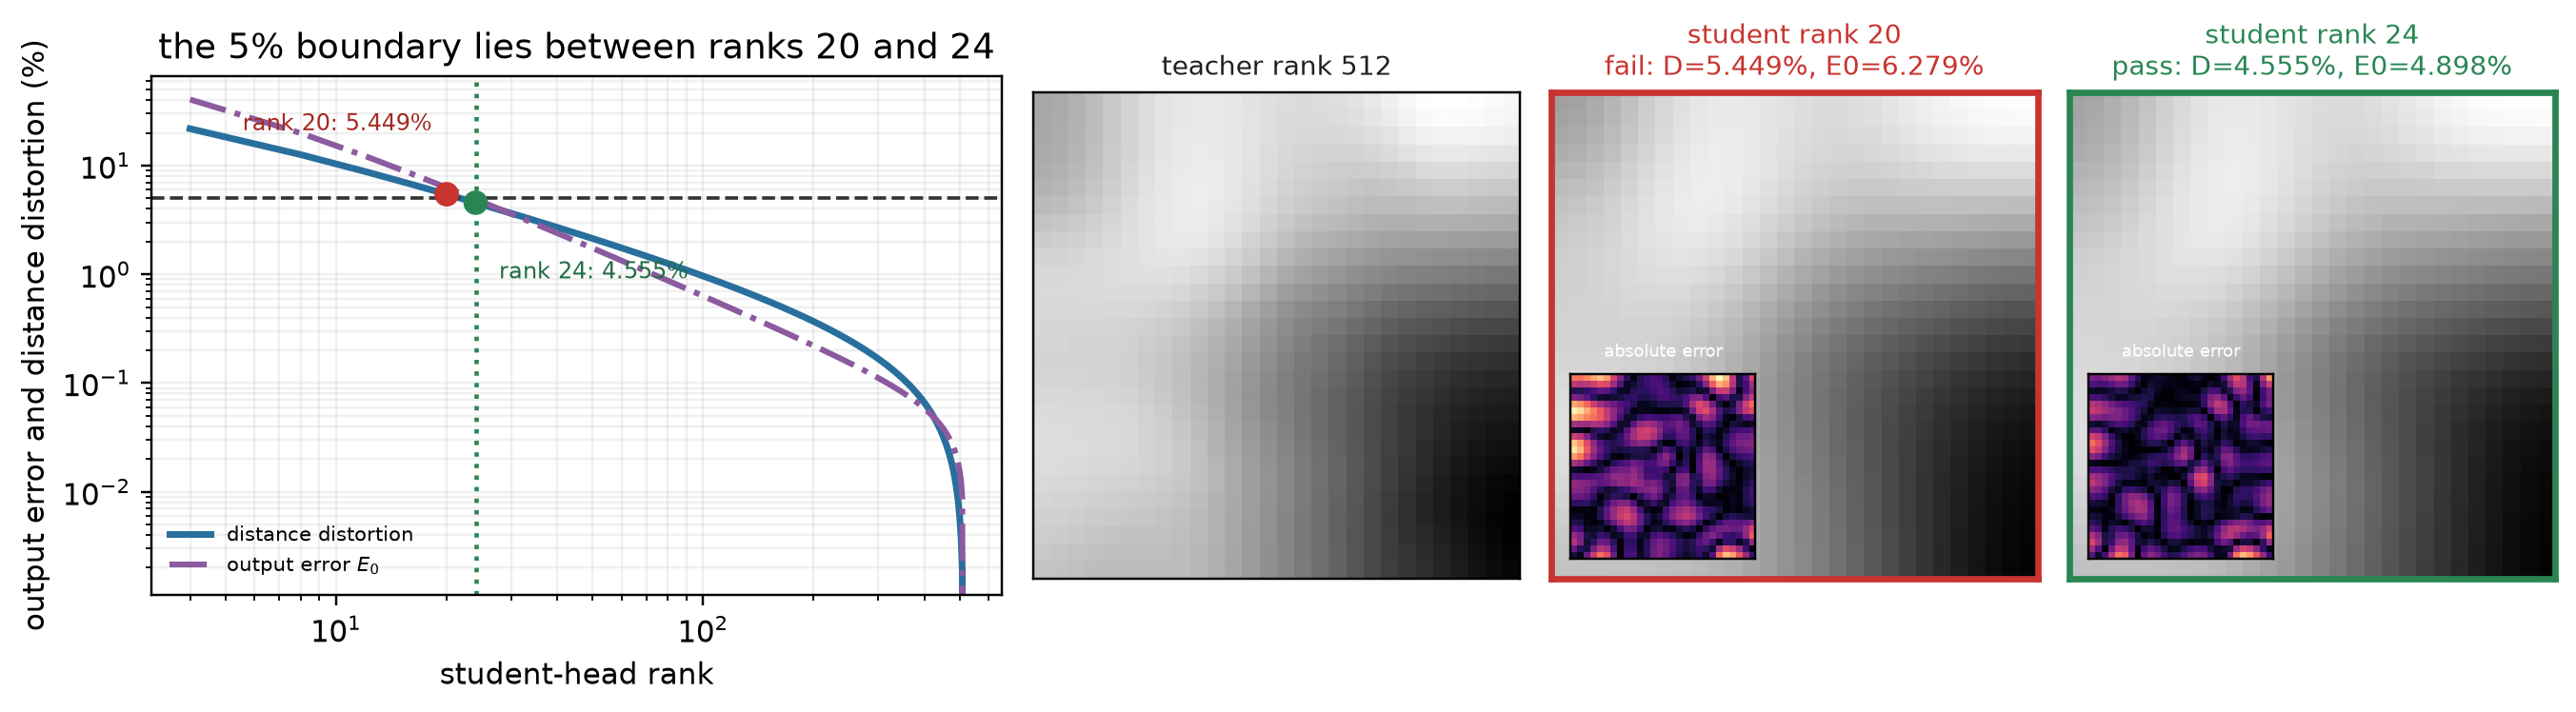
\includegraphics[width=0.98\textwidth]{experiments/lowrank_torus.png}
  \caption{Exact output--geometry frontier.  Both curves are analytic.  Rank
  20 violates the predeclared 5\% output and distance requirements; rank 24
  satisfies both.  Raw images are visually similar, so the insets show
  absolute residuals on a common scale.}
  \label{fig:exact-frontier}
\end{figure*}

\begin{table}[t]
  \centering
  \small
  \caption{Exact simultaneous thresholds.  The two tolerances are equal in
  each row; compression is the dense-teacher to factorized-student head
  storage ratio.}
  \label{tab:exact-thresholds}
  \resizebox{\columnwidth}{!}{\begin{tabular}{rrrrrr}
\toprule
$\eta=\tau$ & Min. rank & Head params. & Compression & $E_0$ & $D_{\mathrm{pair}}$ \\
\midrule
10\% & 16 & 21,520 & 18.69$\times$ & 8.451\% & 6.749\% \\
5\% & 24 & 31,888 & 12.61$\times$ & 4.898\% & 4.555\% \\
2\% & 56 & 73,360 & 5.48$\times$ & 1.476\% & 1.886\% \\
1\% & 100 & 130,384 & 3.08$\times$ & 0.631\% & 0.965\% \\
\bottomrule
\end{tabular}
}
\end{table}

\paragraph{A sharp five-percent result.}
For five retained frequency blocks (rank 20), Proposition
\ref{prop:exact-rank-law} gives
\begin{equation}
 E_{0,5}=6.2788\%,
 \qquad
 D_5=5.4485\%.
\end{equation}
It fails both requirements.  Six blocks (rank 24) give
\begin{equation}
 E_{0,6}=4.8980\%,
 \qquad
 D_6=4.5555\%,
\end{equation}
so the prefix head is feasible.  More importantly, this is not merely the
first point on a chosen truncation curve.  Equation
\eqref{eq:output-rank-lower-bound} gives every shared-trunk rank-23 head the
root-mean-square output lower bound
\begin{equation}
 \inf_{\rank(U)\le23}
 \left(\E_z\norm{(U-W)h(z)}^2\right)^{1/2}
 =5.2772\%>\eta.
\end{equation}
Because the uniform error $E_0$ is at least the RMS error, no rank at most 23
can satisfy \eqref{eq:exact-requirements}.  Rank 24 is therefore the true
minimum over all linear heads sharing this trunk and bias.  It uses $31{,}888$
head scalars, a $12.61\times$ reduction.

Table~\ref{tab:exact-thresholds} shows the joint rate--distortion tradeoff.  At
10\%, output fidelity raises the minimum from the geometry-only rank 12 to
rank 16.  At 1\%, rank 100 is required and compression falls to
$3.08\times$.  This illustrates why output and geometry must both appear in
the definition: geometry alone permits output-different isometries.

The rank-24 result uses the exact Fourier Gram identity, not the more general
Jacobian-error bound in Theorem~\ref{thm:stability}; the latter is a convenient
sufficient condition and can be conservative.  The controlled task therefore
verifies the definition and a sharp structured result, while the next task
tests the generic certificate on learned neural students.

\subsection{Neural Stress Test with Nonconstant Variance}
\label{sec:neural-stress}

The latent region is the two-torus and
\begin{align}
 e(\phi)&=(\cos\phi_1,\sin\phi_1,
             \cos\phi_2,\sin\phi_2),\notag\\
 \phi(z)&=\bigl(z_1+0.05\sin(4z_2),
                 z_2+0.05\sin(4z_1)\bigr),\notag\\
 F_T(z)&=\left(0.9e(\phi(z)),
 0.75+\sqrt{1-0.9^2}\,e(\phi(z))\right).
 \label{eq:warped-teacher}
\end{align}
The last four channels are strictly positive standard deviations, so this
experiment uses the full diagonal-Gaussian $W_2$ formula rather than its
fixed-covariance special case.  The warp has analytic conditioning bounds
$s=0.8$ and $M_1=1.2$.

Students are two-hidden-layer Tanh networks with seven widths, doubling from
4 to 256, and periodic inputs
$(\cos z_1,\sin z_1,\cos z_2,\sin z_2)$.  We train three deterministic seeds
for 2,500 steps.  The baseline minimizes output MSE; the first-order objective
adds five times the mean squared Jacobian error.  We predeclare output
RMSE at most 2\% and distance distortion at most 5\%.

Evaluation uses a fixed $48\times48$ torus grid.  We insert its maximum
Jacobian error into Theorem~\ref{thm:stability}, and compare the resulting
plug-in upper bound with graph distances and 3,072 triplets.  This is a
finite-grid diagnostic: a formal continuum certificate would additionally
require a validated covering/Lipschitz remainder.

\begin{figure*}[t]
  \centering
  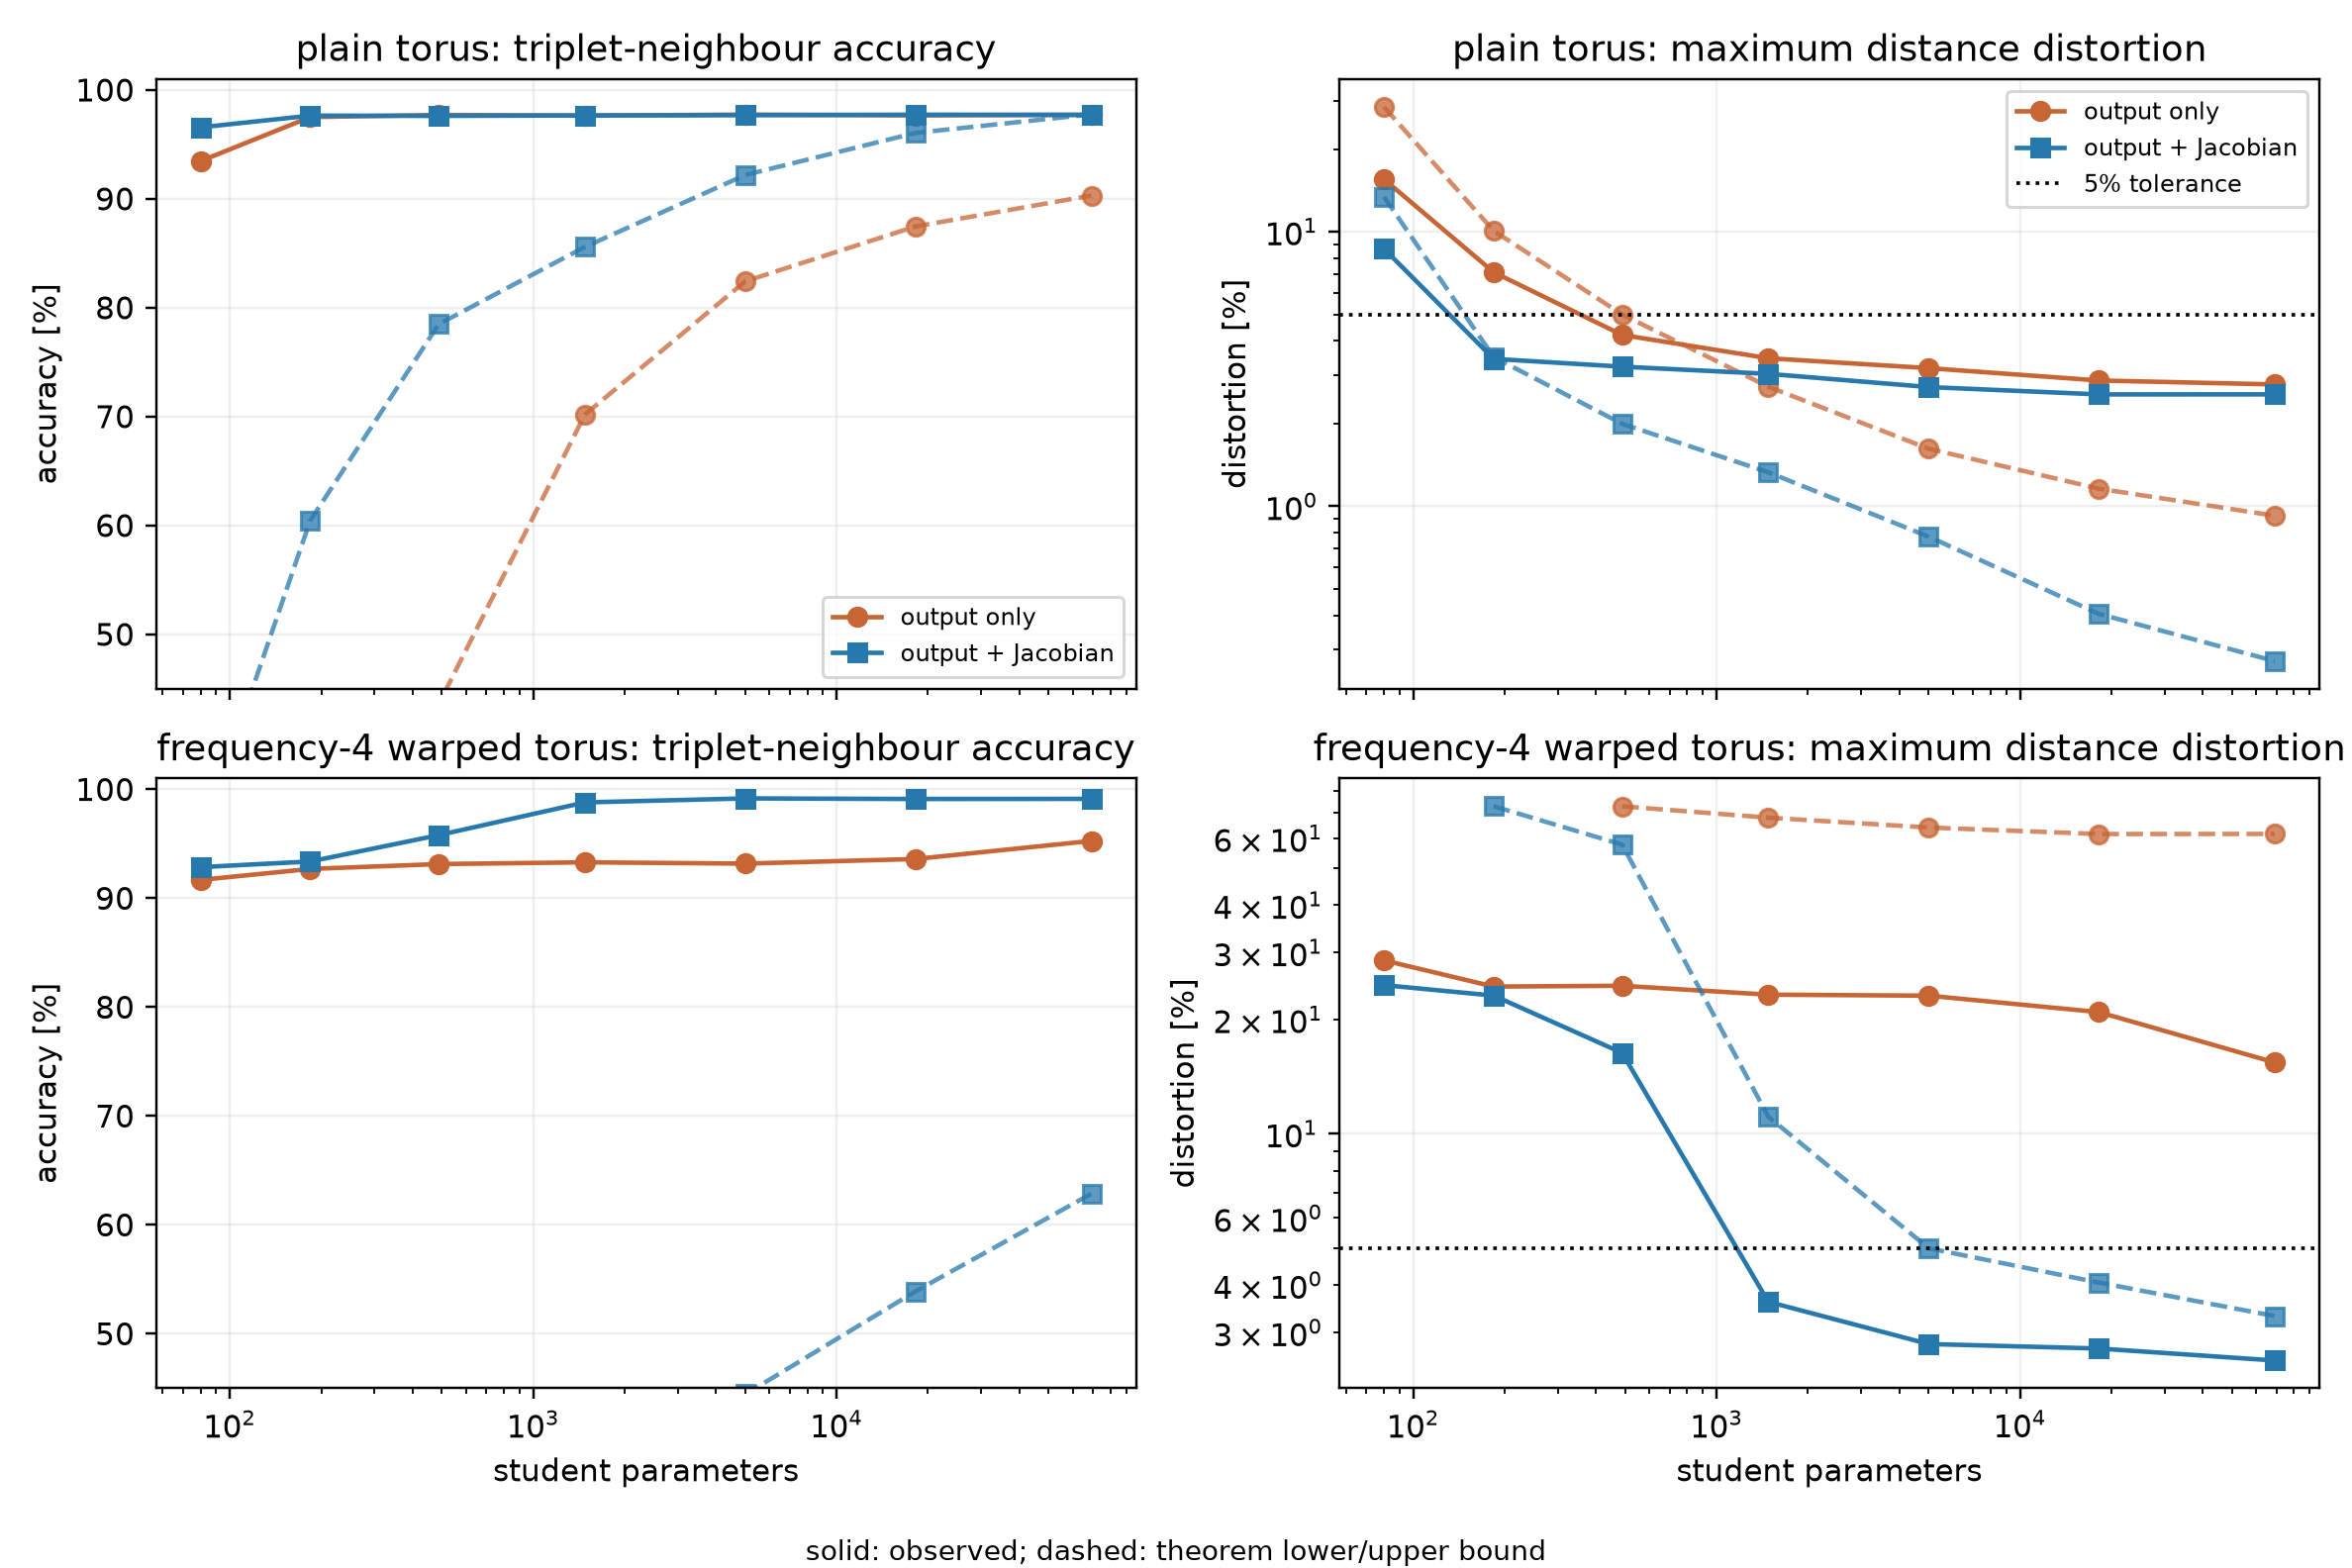
\includegraphics[width=0.94\textwidth]{experiments/distillation_tradeoff.png}
  \caption{Neural capacity sweep (three seeds; curves show their means).
  Solid lines are observed values and dashed lines are finite-grid theorem
  bounds.  On the frequency-4 warped teacher (bottom row), first-order
  distillation crosses the 5\% distance boundary, whereas output-only training
  does not within the tested range.  The plain torus (top row) is included as
  a lower-frequency reference.}
  \label{fig:neural-sweep}
\end{figure*}

On the warped teacher, the largest output-only student has $69{,}128$
parameters and meets the 2\% output requirement (1.308\% RMSE), but its
plug-in distance bound is 61.62\%, its observed maximum pair distortion is
15.41\%, and its triplet agreement is 95.27\%.  It therefore fails for a
specifically geometric reason.  Output--Jacobian training passes for all
three seeds at width 128 ($18{,}184$ parameters): output RMSE is 0.083\%,
$\widehat\varepsilon_1=0.0210$, the theorem bound is 4.06\%, observed maximum
pair distortion is 2.72\%, and triplet agreement is 99.12\%.  Across all 84
runs, observed local metric distortion never exceeds the corresponding
plug-in $\delta$.  These results do not prove an optimizer-independent lower
bound; they show that the quantity used by the theorem is learnable and that
output fitting alone need not learn it.

\subsection{Real-Data VAE Head Compression}
\label{sec:realdata}

\paragraph{Setup.}
We train separate two-dimensional Gaussian VAEs \cite{kingma2014} on seeded
subsets of 30,000 MNIST \cite{lecun1998} and FashionMNIST \cite{xiao2017}
training images for 12 epochs.  Both use the architecture in
Figure~\ref{fig:architecture}: a two-layer width-64 Tanh decoder trunk
$h:\R^2\to\R^{64}$ and a $784\times64$ affine mean head with fixed
observation covariance.  We freeze encoder, trunk, and bias and replace only
$W$.  This is decoder-head compression, not whole-VAE compression.

We compare ordinary SVD ($C=I$), value-weighted SVD
($C=\E[hh^{\trans}]+\rho I$), and value--Jacobian SVD using
\eqref{eq:jet-covariance}.  For each dataset, $C$ is fitted on 4,096 training
posterior means.  The Jacobian covariance is assigned four times the trace of
the value covariance, fixed before test-rank evaluation.

All 64 ranks are evaluated on 4,000 official-test posterior means.  We report
$\widehat D_{\rm loc}$, the maximum generalized-eigenvalue length error on a
fixed 1,536-point subset, and 6,000 local teacher-$W_2$ chord triplets.  Rank
selection and reporting use this same finite subset.  The crossings are
therefore sampled thresholds, not held-out continuum certificates.

\begin{table*}[t]
  \centering
  \small
  \caption{Sampled 5\% local-geometry crossings.  ``Triplet'' is local
  teacher-$W_2$ chord-order agreement, not class-label accuracy or intrinsic
  geodesic accuracy.  A factorized head larger than the dense head falls back
  to dense storage, hence $1.00\times$.}
  \label{tab:realdata-crossings}
  \resizebox{0.98\textwidth}{!}{\begin{tabular}{llrrrr}
\toprule
Dataset & Method & Rank fail $\to$ pass & $\widehat D_{\rm loc}$ fail $\to$ pass & Head reduction & Triplet \\
\midrule
MNIST & ordinary SVD & 59 $\to$ 60 & 6.79\% $\to$ 4.94\% & 1.00$\times$ & 99.32\% \\
 & value-weighted SVD & 11 $\to$ 12 & 5.12\% $\to$ 4.20\% & 4.65$\times$ & 99.97\% \\
 & value + Jacobian SVD & 11 $\to$ 12 & 5.20\% $\to$ 4.17\% & 4.65$\times$ & 99.95\% \\
\addlinespace
FashionMNIST & ordinary SVD & 62 $\to$ 63 & 5.44\% $\to$ 2.92\% & 1.00$\times$ & 99.98\% \\
 & value-weighted SVD & 12 $\to$ 13 & 7.93\% $\to$ 4.83\% & 4.32$\times$ & 99.93\% \\
 & value + Jacobian SVD & 12 $\to$ 13 & 7.49\% $\to$ 3.36\% & 4.32$\times$ & 100.00\% \\
\bottomrule
\end{tabular}
}
\end{table*}

On MNIST, ordinary SVD first passes at rank 60
($4.944\%$; rank 59 gives $6.794\%$), while both covariance-aware methods pass
at rank 12 ($4.196\%$ and $4.173\%$).  Rank 12 reduces the head from 50,960 to
10,960 parameters ($4.65\times$) and the full decoder from 55,312 to 15,312
($3.61\times$).  FashionMNIST independently reproduces the separation:
ordinary SVD first passes at rank 63, while both weighted methods pass at rank
13.  The value--Jacobian student has $3.359\%$ distortion and reduces the head
to 11,808 parameters ($4.32\times$), or the decoder to 16,160
($3.42\times$).  Their local chord-triplet agreements are 99.95\% and 100.00\%.

The Jacobian term does not reduce the crossing rank relative to value weighting
on either dataset.  It gives slightly more margin at the crossing, but it does
not dominate at every aggressive rank: the objectives allocate limited rank
differently.  The robust real-data conclusion is therefore that calibration
covariance produces the large rank reduction, while the Jacobian component
targets geometry within that weighted family.

\begin{figure*}[t]
  \centering
  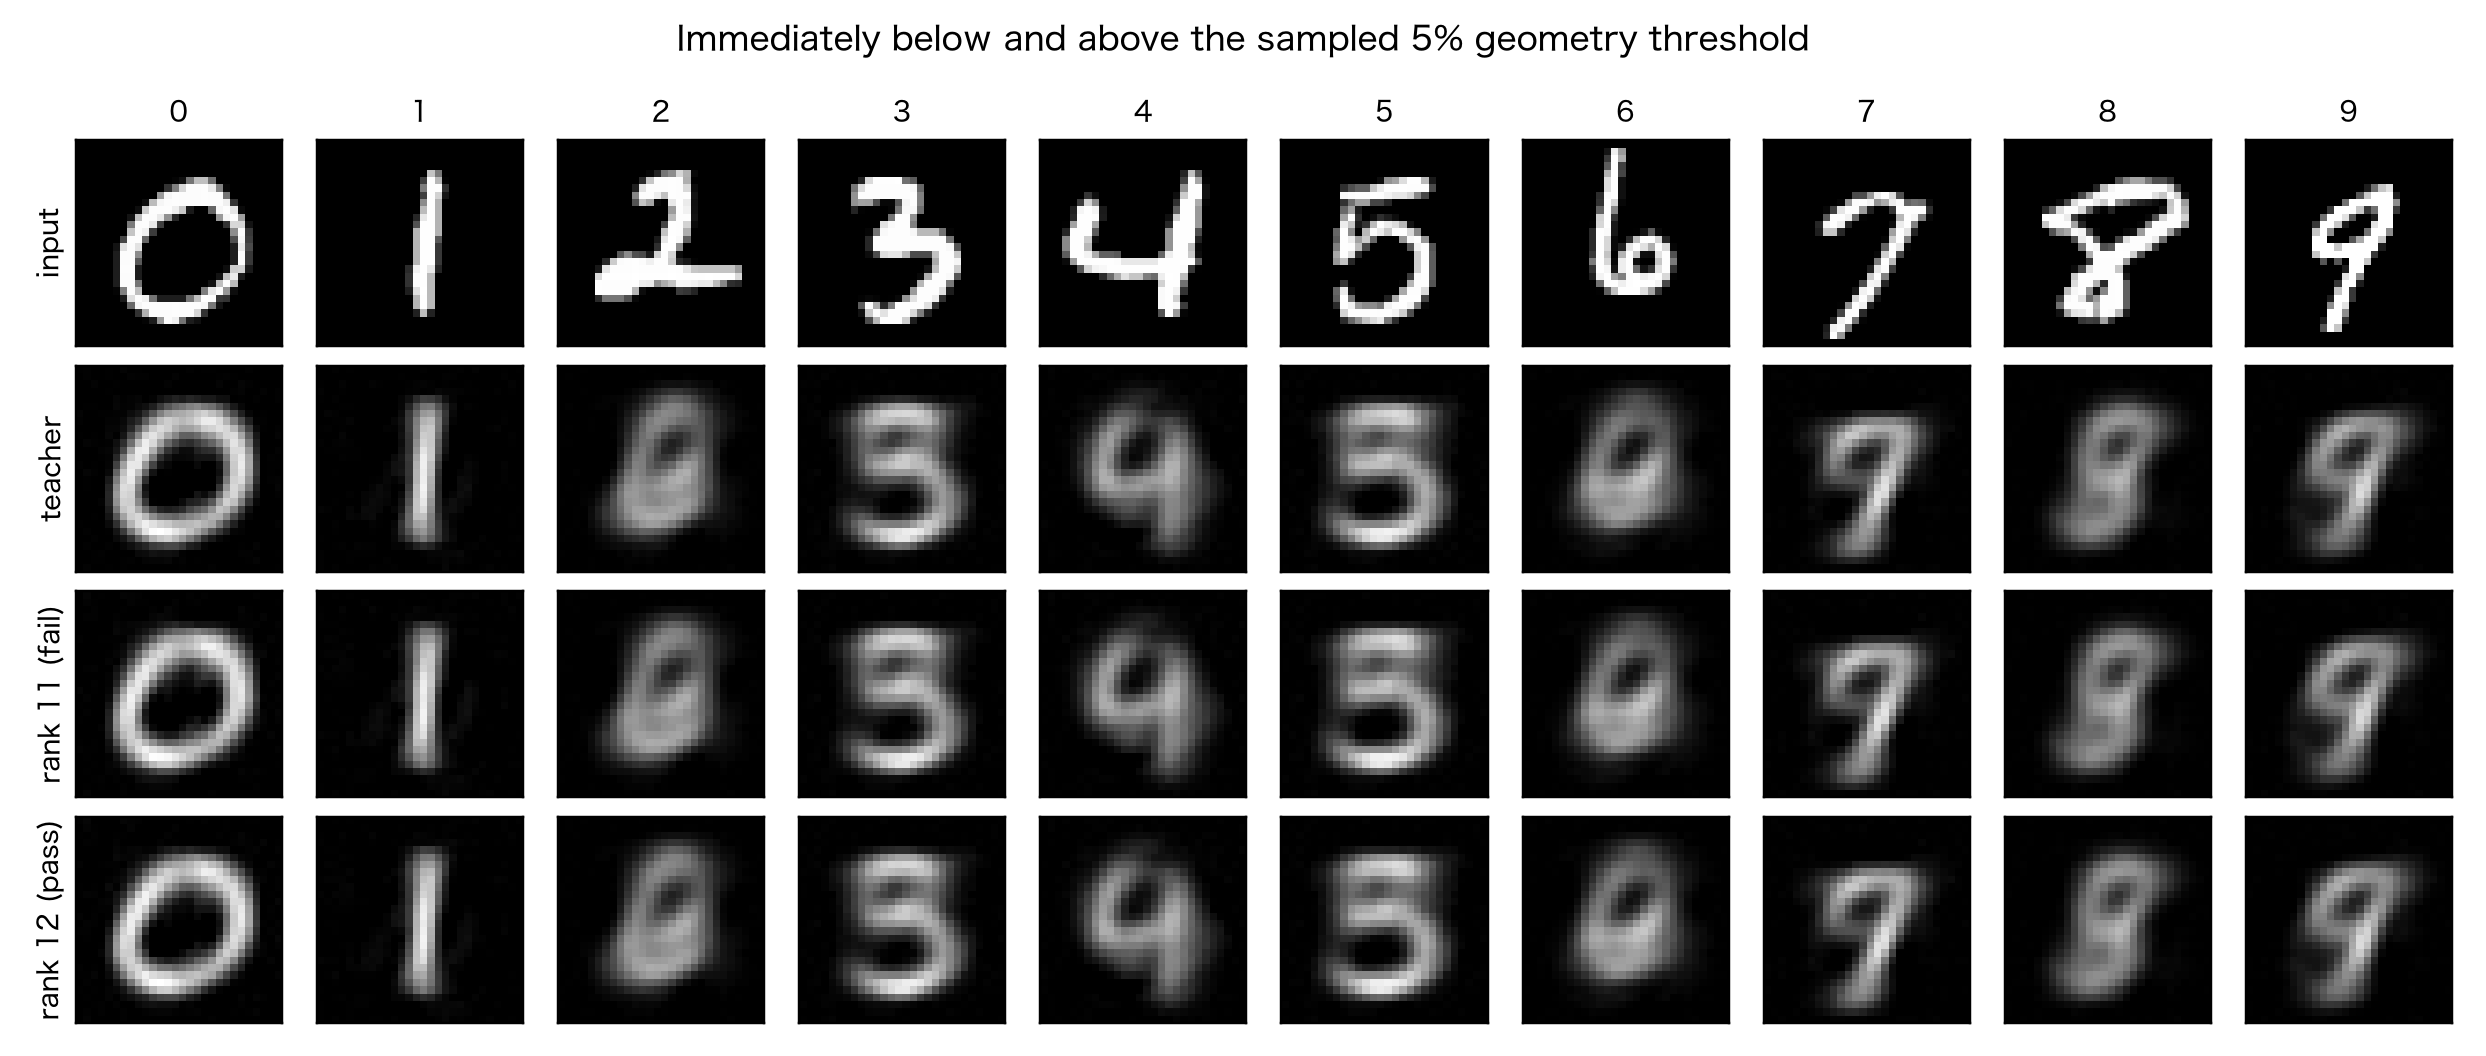
\includegraphics[width=0.96\textwidth]{experiments/mnist_low_rank_images.png}
  \vspace{1mm}
  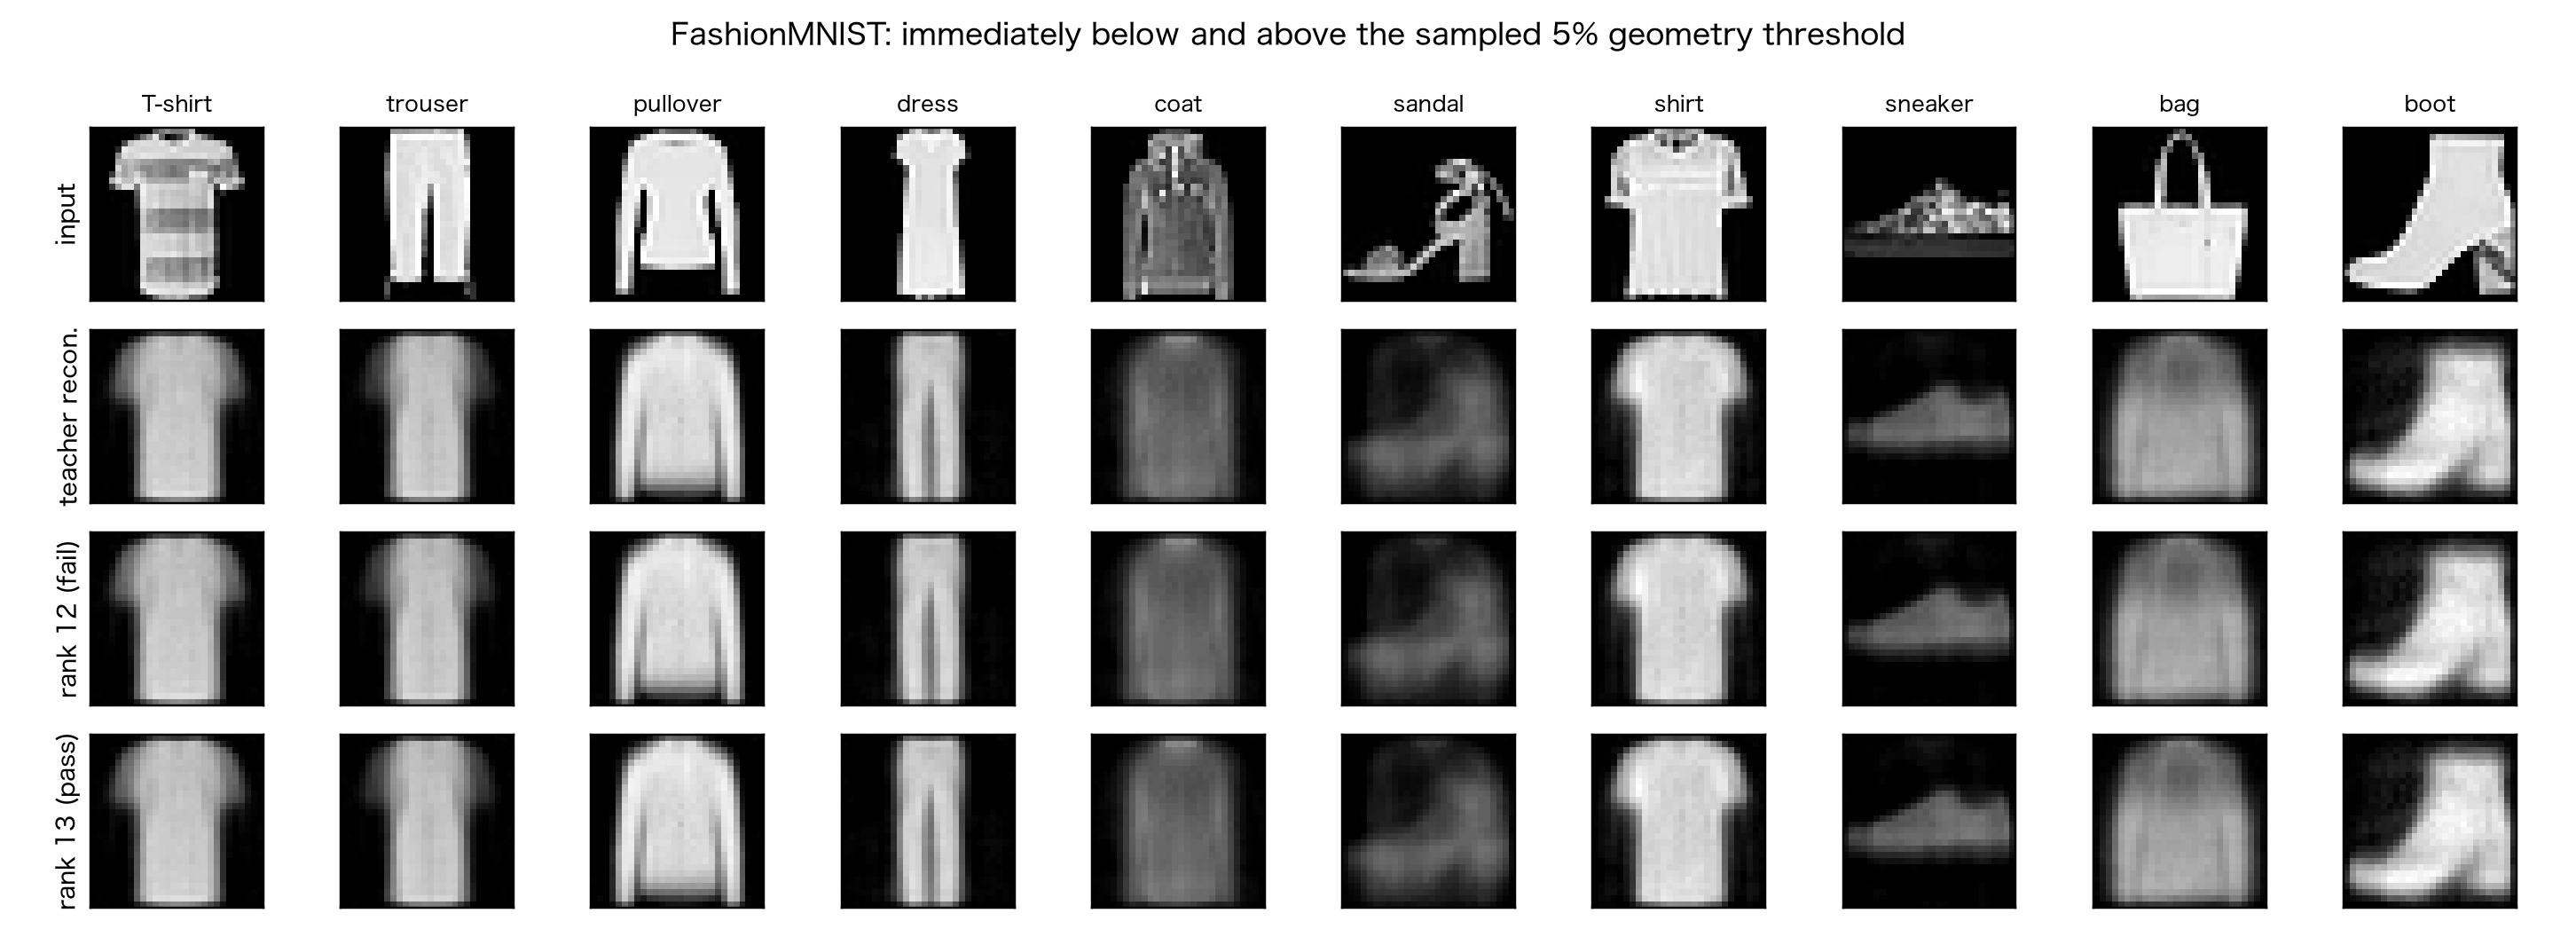
\includegraphics[width=0.99\textwidth]{experiments/fashion_mnist_low_rank_images.png}
  \caption{Official-test inputs, frozen-teacher reconstructions, and
  value--Jacobian students immediately below and above each sampled 5\%
  threshold.  MNIST uses ranks 11/12 and FashionMNIST uses 12/13.  The adjacent
  images can look nearly identical while lying on opposite sides of a
  derivative-defined geometric criterion.}
  \label{fig:realdata-images}
\end{figure*}

\subsection{Straight Lines versus Numerical Intrinsic Paths}
\label{sec:geodesic-visualization}

We next make the preserved geometry visible.  Endpoints are posterior means,
and the path remains inside a prespecified evaluation rectangle: coordinate-
wise 0.5--99.5\% quantiles of the fixed 3,000-image official-test posterior-
mean pool, with a 3\% margin.  This rectangle is a numerical trust region, not
the support of a Gaussian posterior.  Endpoint pairs use different labels,
central 5--95\% codes, reconstruction errors below the 75th percentile, and
moderate Mahalanobis separation.

For 49 knots with fixed endpoints, we minimize the midpoint discretization of
the teacher pullback energy,
\begin{equation}
 \begin{aligned}
 E_K(c)&=(K-1)\sum_{k=0}^{K-2}
 \dot z_k^{\trans}G_T(\bar z_k)\dot z_k,\\
 \dot z_k&=z_{k+1}-z_k,
 &\bar z_k&=\frac{z_{k+1}+z_k}{2}.
 \end{aligned}
 \label{eq:discrete-geodesic-energy}
\end{equation}
Three initial paths are optimized for 700 deterministic Adam steps, and final
length is recomputed separately by fine metric quadrature.  The displayed path
is additionally resampled at equal teacher arc length.  We call the result a
\emph{numerical geodesic candidate}: global optimality is not certified.  It
is an intrinsic path constrained to the frozen decoder family, not an ambient
Wasserstein displacement geodesic and not a path on the unknown true data
manifold.

We evaluate 100 fixed, randomly sampled, endpoint-disjoint pairs per dataset.
The diagnostic pair in each figure is selected using only the straight path's
decoded-step nonuniformity and chord excess, before computing its candidate.
Table~\ref{tab:geodesics} reports conditional percentile pair-bootstrap
intervals over 2,000 resamples; they measure endpoint-pair variation for one
frozen teacher, not teacher-training or population uncertainty.  Across the
200 reported teacher candidates, the relative 8-versus-16 subdivision length
gap is below $2\times10^{-6}$, and none touches the evaluation-box boundary.
On a fourfold densification of every path, the sampled minimum eigenvalues of
$G_T$ are 3.29 (MNIST) and 4.49 (FashionMNIST), while the largest sampled
condition numbers are 6.30 and 7.14.  This finite check supports, but does not
certify over the continuum, the Riemannian interpretation.

\begin{figure*}[t]
  \centering
  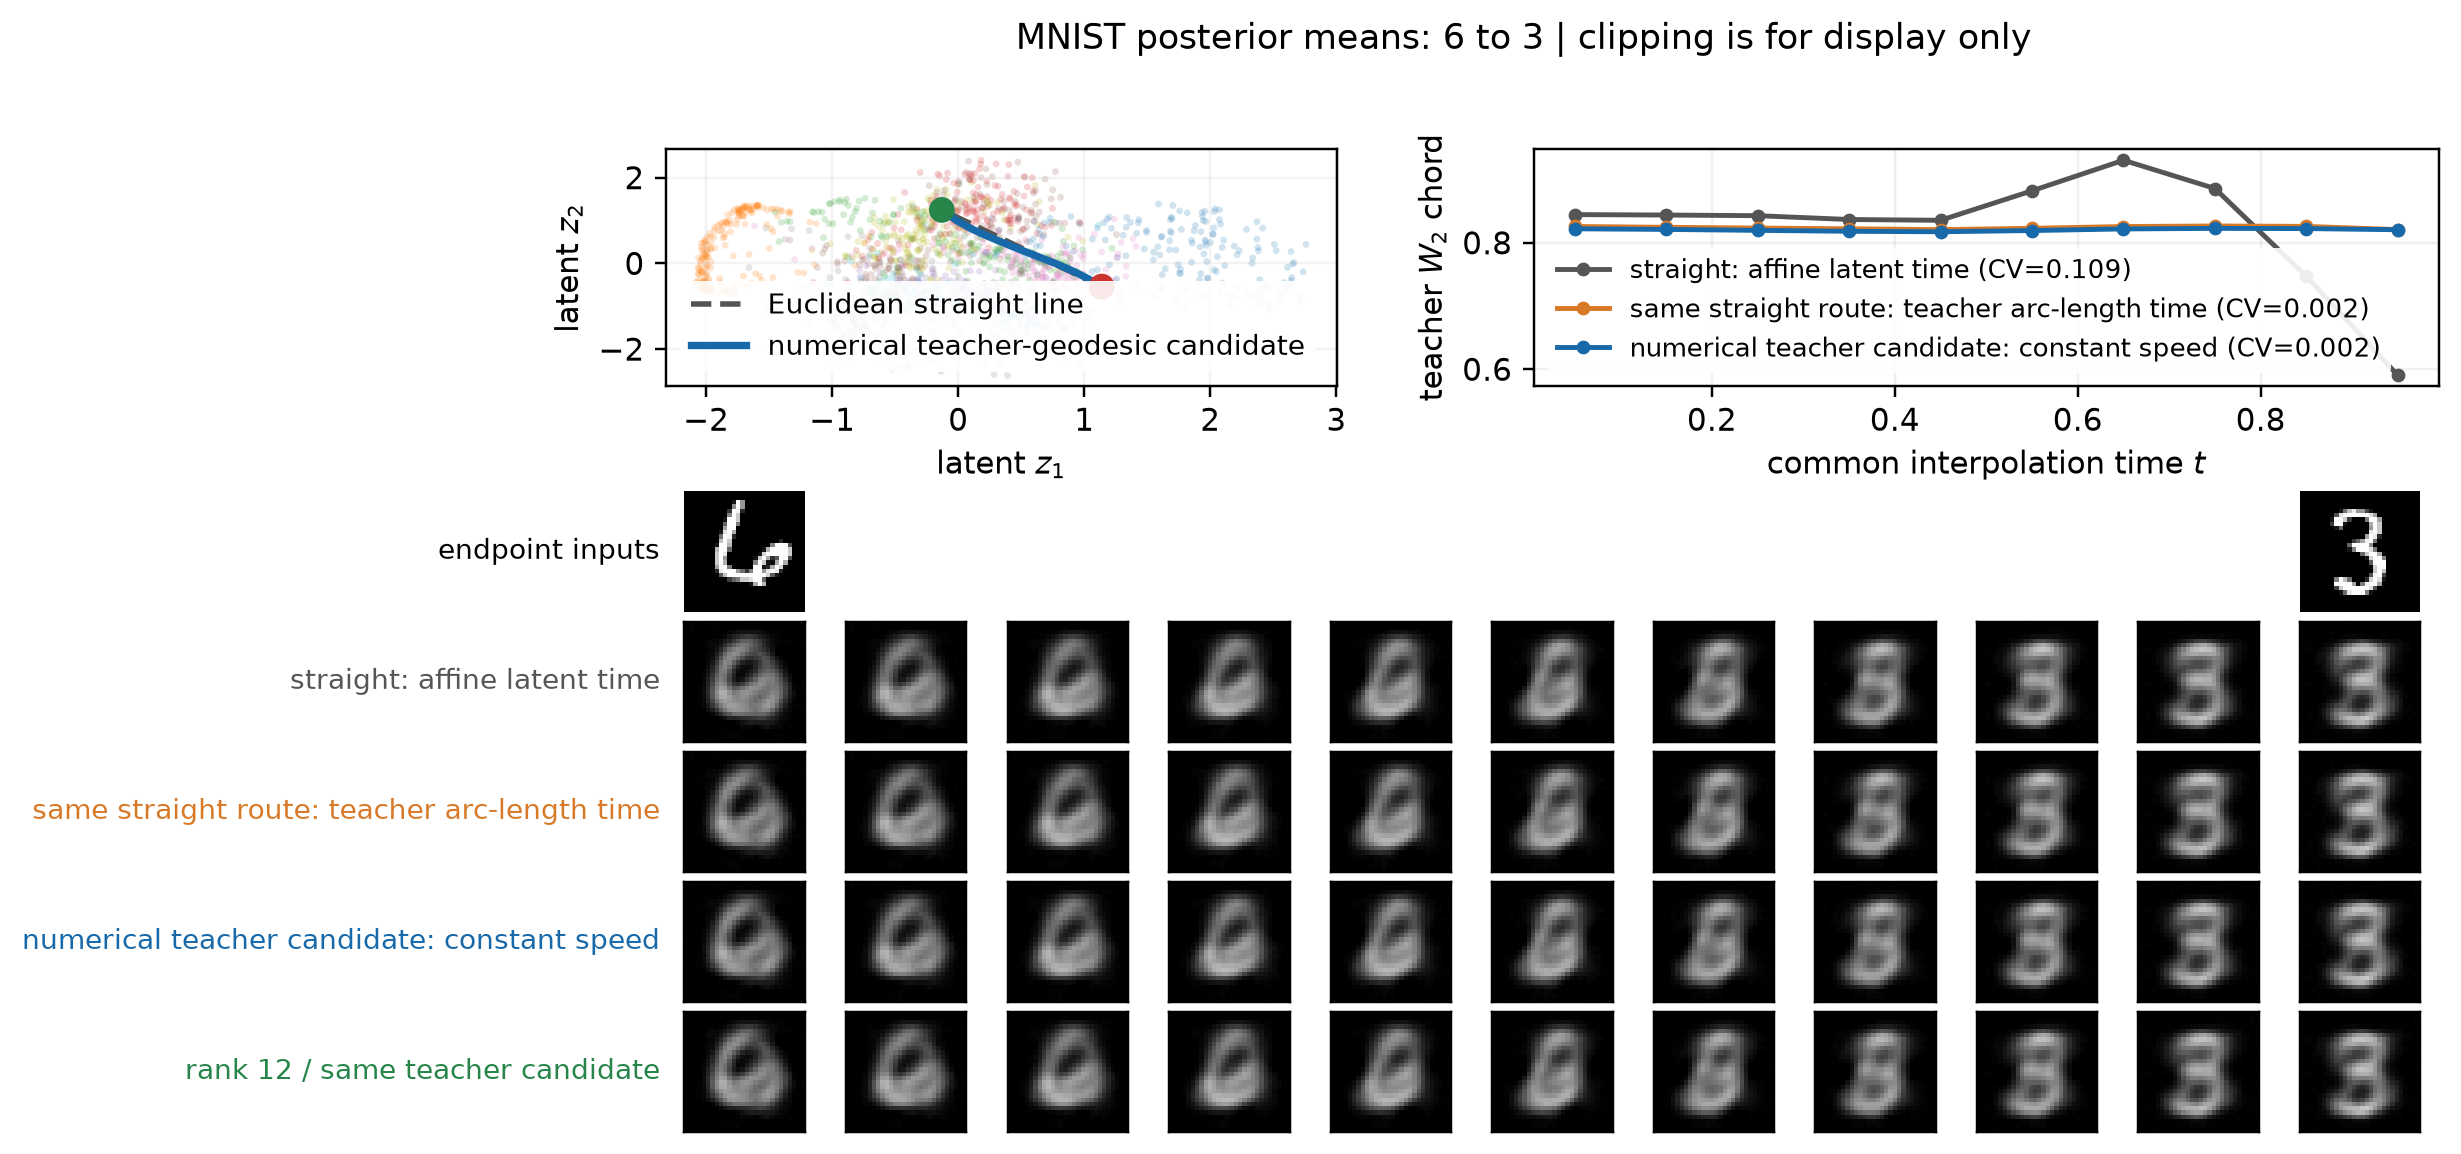
\includegraphics[width=0.96\textwidth]{experiments/mnist_geodesic_interpolation.png}
  \vspace{2mm}
  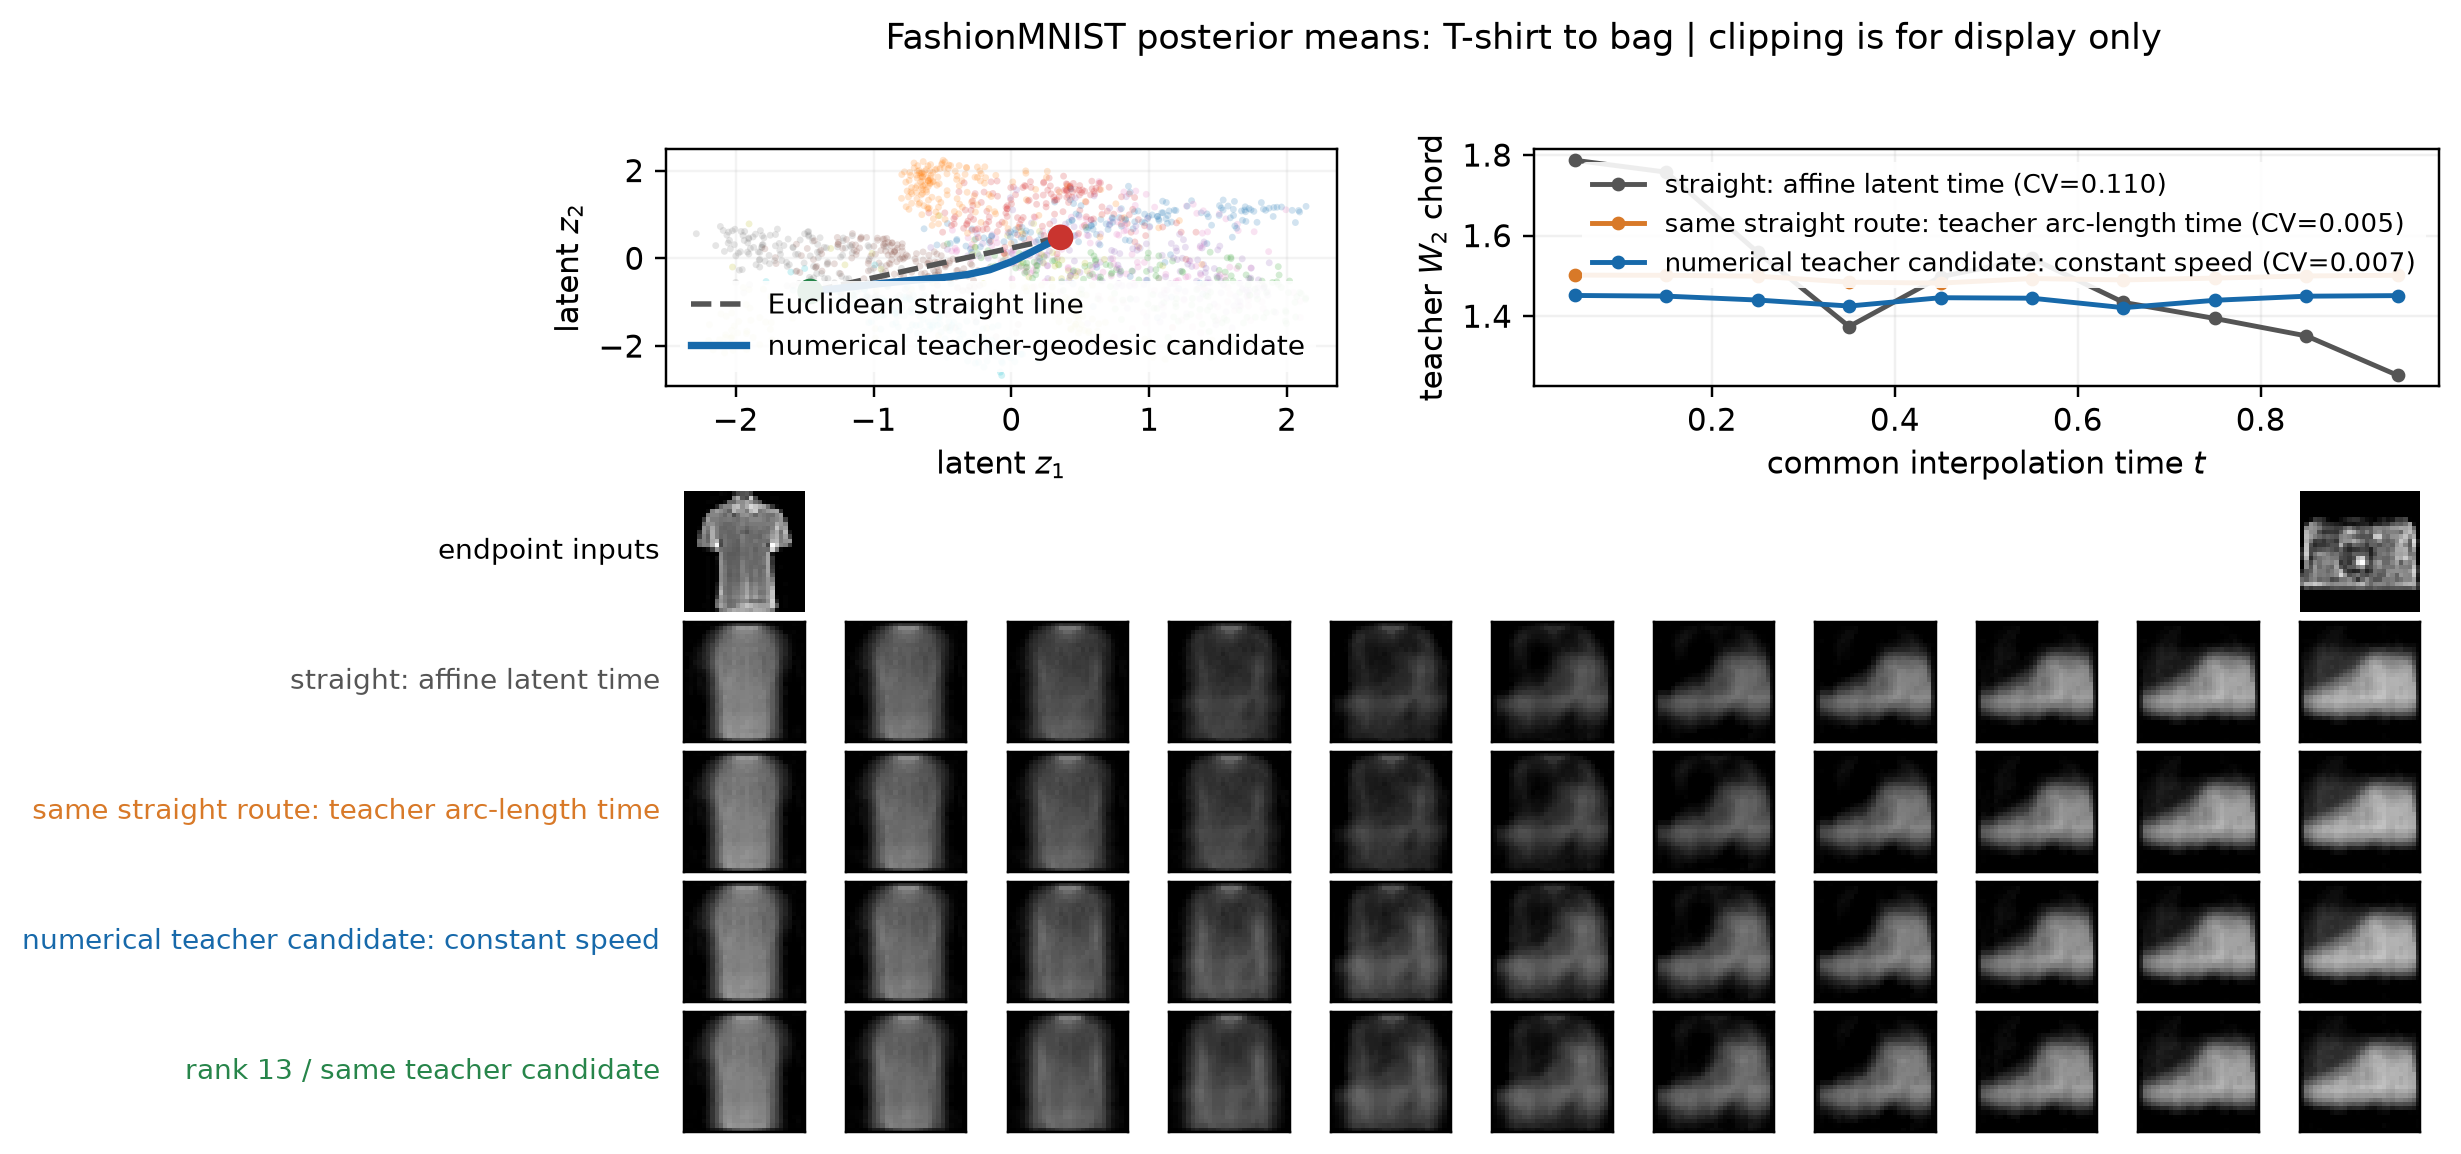
\includegraphics[width=0.96\textwidth]{experiments/fashion_mnist_geodesic_interpolation.png}
  \caption{Input endpoints and decoded interpolation sequences.  The first
  decoded row uses an affine latent clock; the second uses the identical
  straight route at constant teacher arc length; the third changes the route
  to the numerical teacher-geodesic candidate; the last decodes those same
  latent frames with the passing compressed student.  Top panels show the
  latent routes and exact fixed-covariance Gaussian $W_2$ chords between
  displayed frames.  Clipping to $[0,1]$ is for display only.}
  \label{fig:realdata-geodesics}
\end{figure*}

\begin{table*}[t]
  \centering
  \small
  \caption{Numerical intrinsic-path results over fixed endpoint pairs.  Straight
  excess is $L_T(c_{\rm line})/L_T(\widehat\gamma_T)-1$.  Student path error
  measures curve-length error for the passing rank-12/rank-13 student along
  the same teacher path.  Intervals are conditional percentile pair-bootstrap
  intervals for one frozen teacher.  All bracketed values are percentages.}
  \label{tab:geodesics}
  \resizebox{0.94\textwidth}{!}{\begin{tabular}{lrrrr}
\toprule
Dataset & Pairs & Straight excess median [IQR] & 95\% pair-bootstrap CI & Student path error med. / max \\
\midrule
MNIST & 100 & 0.60\% [0.18, 1.60] & [0.43, 0.76] & 0.11\% / 0.36\% \\
FashionMNIST & 100 & 0.75\% [0.31, 1.42] & [0.63, 1.08] & 0.10\% / 0.22\% \\
\bottomrule
\end{tabular}
}
\end{table*}

The median straight-line excess is 0.60\% on MNIST and 0.75\% on
FashionMNIST, with maxima 10.90\% and 4.63\%.  The passing students preserve
curve length along the same teacher candidates with median errors only 0.11\%
and 0.10\%
(maxima 0.36\% and 0.22\%).  In the displayed FashionMNIST pair, the teacher
straight route has length 15.027 and the candidate has length 14.524, a 3.47\%
reduction.  Uniform latent time has adjacent-frame $W_2$ coefficient of
variation 0.110; arc-length reparameterization reduces it to 0.005, and the
numerical candidate has 0.007.  Thus the plot separates a speed effect from a
genuine route change.  The student row uses exactly the same latent codes as
the teacher row.  A student-optimized candidate is computed only for the
displayed pair and reported as a candidate-length audit in the detailed CSV;
it is not part of the 100-pair statistic.

\section{Discussion and Limitations}

\paragraph{What is genuinely minimal?}
The exact task proves rank 24 minimal over every linear head sharing the stated
trunk and bias because it combines a universal rank-output lower bound with a
feasible distance-preserving head.  Theorem~\ref{thm:rank-distillation}
separately gives the exact optimum of the declared first-order distillation
loss at every rank.  Neither statement excludes a different nonlinear trunk
from representing the same teacher behavior with fewer parameters.

\paragraph{Certificates versus sampled tests.}
Theorem~\ref{thm:stability} is a continuum statement when valid global bounds
on $s$, $M_1$, and $\varepsilon_1$ are available.  The analytic image task has
exact global quantities.  The neural sweep and both image datasets replace
suprema by finite sets and are labeled accordingly.  A covering argument,
interval bounds, or a verified Lipschitz remainder is required before calling
those curves global certificates.

\paragraph{Parameters, bits, and deployment.}
An unrestricted real number can encode unbounded information, so universal
parameter-count lower bounds require encodable or quantized weights.  For
deployment, \eqref{eq:min-safe-size} should minimize stored bits and include
rank-factor indices and precision.  Quantization contributes an additional
Jacobian perturbation to Theorem~\ref{thm:stability}.

\paragraph{Teacher-relative geometry.}
On real data, compression can preserve a frozen teacher; it cannot certify
that the teacher recovered the true data manifold.  Both VAEs have one teacher
seed and a deliberately restrictive two-dimensional code; teacher PSNR is
13.19 dB on MNIST and 14.78 dB on FashionMNIST.  They are transparent
applications rather than state-of-the-art image models.  Fixed covariance
makes $W_2$ the Euclidean mean-image special case; the warped-torus experiment
covers learned, nonconstant standard deviations.  Full covariance would
require Bures--Wasserstein geometry.

\paragraph{Numerical paths.}
The displayed paths are local multistart minimizers inside a coordinate-
dependent evaluation rectangle.  Quadrature and boundary diagnostics rule out
the simplest numerical failures but do not prove a global geodesic.  A grid
initialization, knot-refinement study, rectangle-expansion sensitivity, and
perceptual output metric would strengthen claims about interpolation quality.

\paragraph{Scope.}
We study distance and retrieval.  Curvature stability would require
second-order control, and nonlinear variance heads would require constrained
or nonlinear compression.  Stronger empirical claims need multiple teacher
seeds, an independent validation/test split for rank selection, a
Jacobian-weight ablation, and datasets beyond $28\times28$ grayscale images.

\section{Conclusion}

The capacity of a compressed decoder should be defined by the behavior it must
preserve.  For Gaussian decoders, optimal transport turns that behavior into
a pullback metric.  We derived a sufficient scaling from simultaneous value
and derivative approximation, converted metric distortion into triplet
accuracy, and solved fixed-trunk rank-constrained first-order distillation by
covariance-whitened SVD.  The exact image task gives a proof-level answer:
with 5\% output and distance tolerances, rank 23 and below are impossible,
rank 24 is feasible, and the head is $12.61\times$ smaller.  A nonconstant-
variance neural stress test and sampled MNIST/FashionMNIST frontiers show how
the same criterion guides training and deployment.  Input--output panels and
straight-versus-intrinsic decoded sequences then expose what the preserved
geometry does.  The result is not a universal minimum neural network; it is a
reproducible way to turn ``how small?'' into a mathematical constraint and an
auditable accuracy boundary.

\section*{Reproducibility}

The scripts, fixed seeds, CSV results, tables, figures, and both language
editions are regenerated with
\begin{verbatim}
make paper-all
\end{verbatim}
Dataset downloads and the learned MNIST/FashionMNIST teacher checkpoints are
cached locally and excluded from version control.
